\documentclass[../main.tex]{subfiles}


\begin{document}


\subsection{Main Figures}

\begin{figure}[H]
	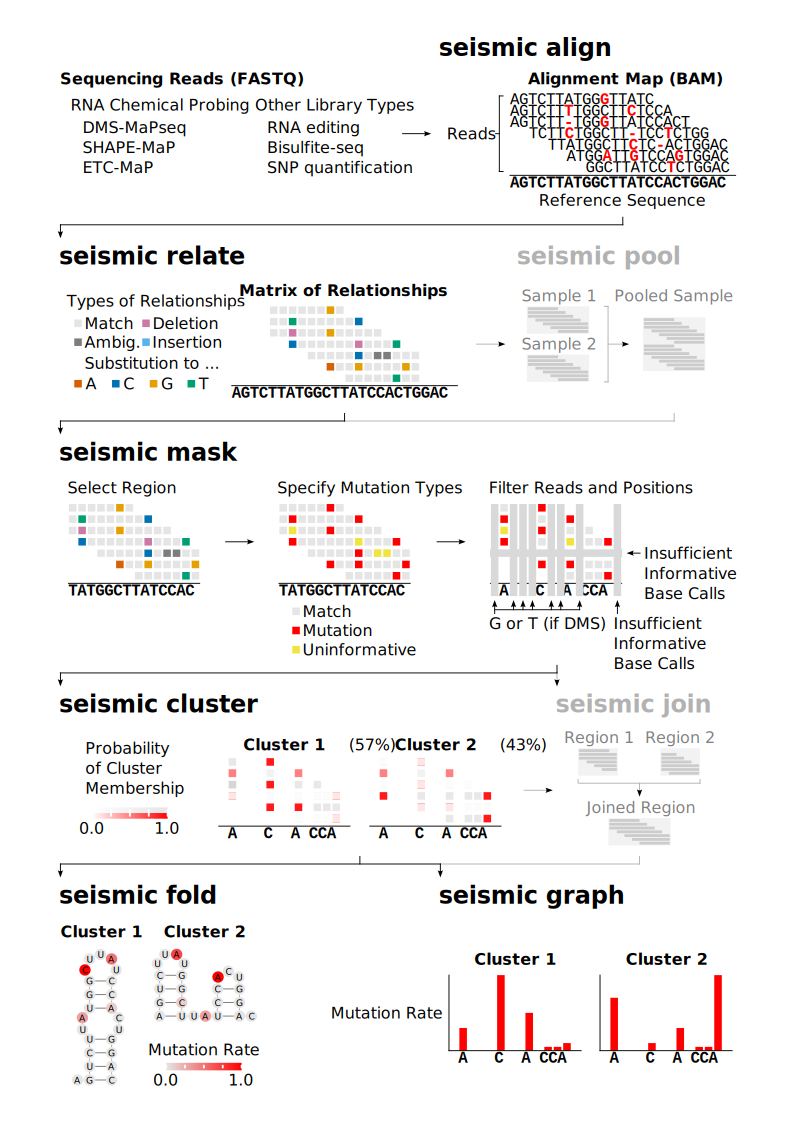
\includegraphics[width=\textwidth]{Figure_1.pdf}
	\caption{\textbf{SEISMIC-RNA processes sequencing reads into predicted RNA structures.} (Continued on next page.)}
	\label{wf}
\end{figure}
\addtocounter{figure}{-1}
\pagebreak
\begin{figure}[H]
	\caption[]{(Continued from previous page.) As input, SEISMIC-RNA accepts sequencing reads from RNA mutational profiling experiments (e.g. DMS-MaPseq~\cite{Zubradt2016} , SHAPE-MaP~\cite{Siegfried2014}, ETC-MaP~\cite{Douds2024}) or other experiments whose readouts are point mutations. SEISMIC-RNA first aligns the reads to the reference sequence of each RNA using Bowtie~2~\cite{Langmead2012}. Next, it determines the relationship (i.e. match, substitution, deletion, insertion) between each read and each position in the reference. It marks low-quality base calls and deletions/insertions in repetitive sequences as ambiguous. It also clips 4 bases from both ends of each read to correct bias against mutations during local alignment. Optionally, users can then pool together multiple samples, such as replicates. Next, SEISMIC-RNA selects relevant data and masks out the remainder: users optionally select a region of the RNA to analyze, specify which relationships to count as mutations, and filter out unusable reads and positions. SEISMIC-RNA then clusters the remaining data to detect alternative RNA structures. Every read is assigned a probability of belonging to each cluster; for each cluster, its proportion is the average of all read probabilities, and its mutation rates are the probability-weighted averages over all reads. Optionally, users can join multiple regions that were masked or clustered individually. SEISMIC-RNA can then use the mutation rates to predict the RNA structure corresponding to each cluster using RNAstructure~\cite{Reuter2010}, as well as generate 13 types of graphs, such as bar graphs of the mutation rates. This entire workflow (except pool and join) can be run with one command: ``seismic wf".}
\end{figure}

\begin{figure}[H]
	\includegraphics[width=\textwidth]{Figure_2.pdf}
	\caption{\textbf{Reads with nearby mutations are underrepresented, producing false clusters unless corrected for.} (Continued on next page.)}
	\label{mutation-gap}
\end{figure}
\addtocounter{figure}{-1}
\pagebreak
\begin{figure}[H]
	\caption[]{(Continued from previous page.) \textbf{(A)} Reads whose two closest mutations have a gap less than 4~nt are underrepresented in DMS-MaPseq data~\cite{Morandi2021} compared to the theoretical expectation if mutations occurred independently. \textbf{(B)} Underrepresentation of reads with nearby mutations can cause false clusters. For an RNA that forms a single structure, reads with two mutations less than 4~nt apart will occur rarely in sequencing data. Thus, the two mutations will be anti-correlated, so a naive clustering algorithm will falsely create a cluster for each mutation. \textbf{(C)} We simulated DMS-MaPseq data for 60 random RNA sequences, each with one true cluster, to have bias similar to that of empirical data. Each light trace represents one simulated dataset; the dark traces are the average of all simulated datasets. \textbf{(D)} Without correcting for the bias in mutation gaps, 95\% of simulated datasets incorrectly yielded more than one cluster. With SEISMIC-RNA's bias correction algorithm, all datasets correctly yielded one cluster. \textbf{(E)} In a representative RNA that yielded two clusters without bias correction, position 83 (red) is one of the most frequently mutated positions and is surrounded by six other positions with mutation rates of at least 2\% (orange). Clustering without bias correction assigned reads in which position 83 was mutated predominantly to cluster 2, and reads in which any surrounding position was mutated predominantly to cluster 1, in agreement with panel (B).}
\end{figure}

\begin{figure}[H]
	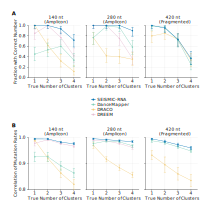
\includegraphics[width=\textwidth]{Figure_3.pdf}
	\caption{\textbf{SEISMIC-RNA is more accurate than similar software.} \textbf{(A)} The fraction of 60 simulations for which SEISMIC-RNA, DanceMapper, DRACO, and DREEM detected the correct number of clusters for each length of RNA and true number of clusters. Error bars show 95\% confidence intervals. \textbf{(B)} The average Pearson correlation between the true mutation rates and those calculated by SEISMIC-RNA, DanceMapper, DRACO, and DREEM for each length of RNA and true number of clusters. Error bars show 95\% confidence intervals.}
	\label{accuracy}
\end{figure}

\begin{figure}[H]
	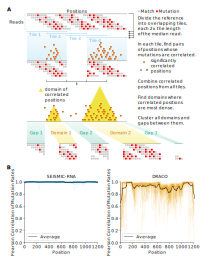
\includegraphics[width=\textwidth]{Figure_4.pdf}
	\caption{\textbf{SEISMIC-RNA clusters long transcripts by first identifying domains that form multiple clusters.} \textbf{(A)} First, SEISMIC-RNA divides a long transcript into tiles, each twice the median read length and overlapping half of each adjacent tile. Within each tile, it finds pairs of positions whose mutations correlate significantly using a hypergeometric test with the Benjamini-Hochberg correction. It then combines correlated pairs from all tiles and identifies domains where pairs are most dense. Finally, it clusters each domain, and optionally each gap between domains. \textbf{(B)} The rolling Pearson correlation (45~nt window size) between the true mutation rates and detected mutation rates for each of the 60 simulated RNAs analyzed with SEISMIC-RNA (transparent blue) or DRACO (transparent orange). The black line shows the average correlation among all simulations.}
	\label{ensembles}
\end{figure}

\begin{figure}[H]
	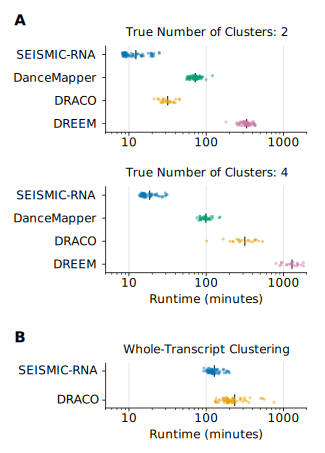
\includegraphics[width=0.548\textwidth]{Figure_5.pdf}
	\caption{\textbf{SEISMIC-RNA is faster than similar software.} \textbf{(A)} Points show the runtime for every simulated dataset of a 280~nt RNA sequence with 200,000 reads whose analysis yielded the true number of clusters. Vertical black bars indicate mean runtimes. For consistency, runtimes of DanceMapper and DRACO include preprocessing with ShapeMapper~2 and RNA Framework, respectively. \textbf{(B)} Similar to (A), but comparing the speed of whole-transcript clustering for the 1,200~nt RNAs.}
	\label{speed}
\end{figure}


\end{document}
